\section{Processo Modelagem}

\begin{frame}	
	\begin{block}{Processo Modelagem}	
			\begin{itemize}
				\item Existem muitos processos para usar na área de big data, um dos mais simples e práticos é o  \href{http://www.bigdatabusiness.com.br/se-voce-se-interessa-por-big-data-precisa-entender-o-crisp-dm/}{\color{blue}{CRISP-DM}} 
			\end{itemize}
			\begin{figure}[!htb]
				\centering	  				
					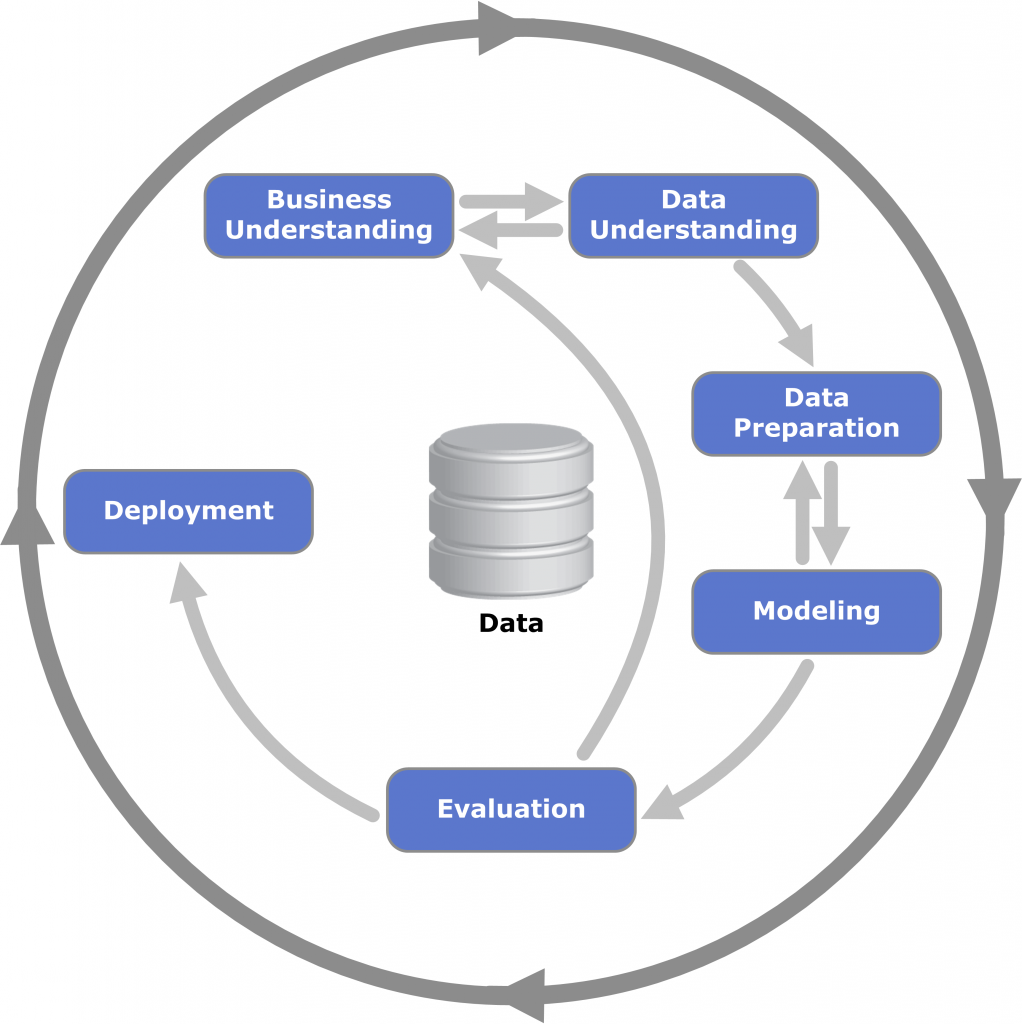
\includegraphics[height=6cm, width = 10cm]{./pic/CRISPDM.png}
				\caption{Processo CRISP-DM}
				\label{fig_brincadeira}
		\end{figure}	
	\end{block}
\end{frame}

\begin{frame}	
	\begin{block}{Processo Modelagem}	
			\begin{itemize}
				\item Entendimento de negócio
				\item Entendimento dos dados
				\item Preparação dos dados 
				\item Modelagem
				\item Avaliação do modelo
				\item Deploy
			\end{itemize}
	\end{block}
\end{frame}

\begin{frame}	
	\begin{block}{Método científico}	
			\begin{figure}[!htb]
				\centering	  				
					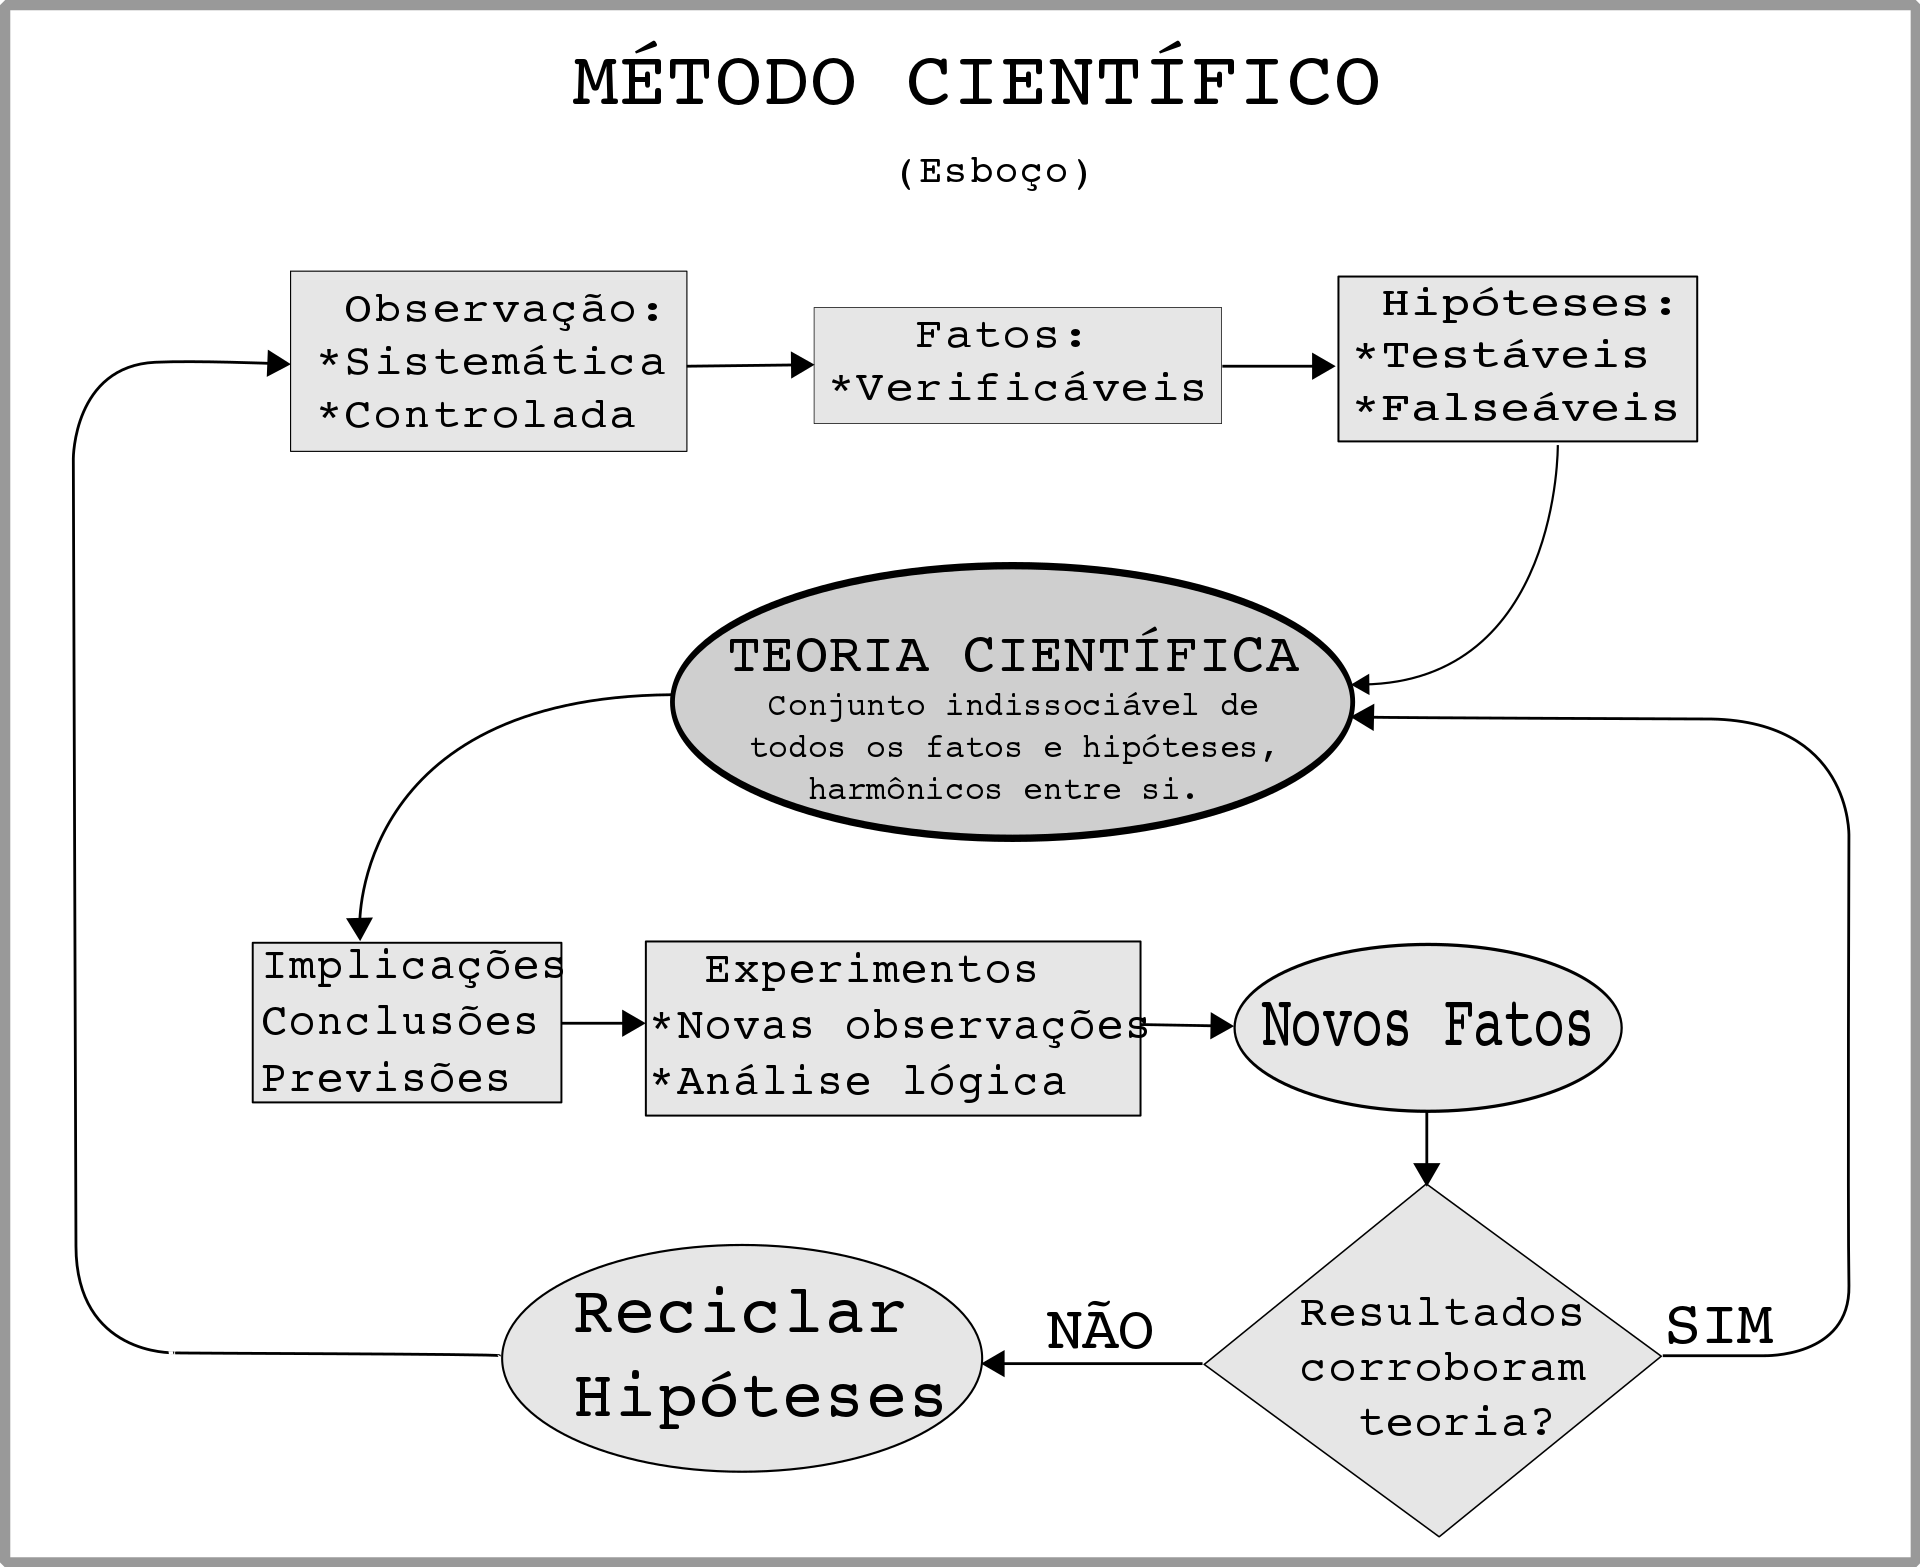
\includegraphics[height=6cm, width = 10cm]{./pic/metodoCientifico.png}
				\caption{Método científico}
				\label{fig_brincadeira}
		\end{figure}	
	\end{block}
\end{frame}

\begin{frame}	
	\begin{block}{Método científico}	
			\begin{itemize}
				\item Então método científico nos impede de cometer erros?
			\end{itemize}
	\end{block}
\end{frame}

\begin{frame}	
	\begin{block}{Método científico}	
			\begin{itemize}
				\item Por que Dirso ficou doente na Argentina em 2018?
			\end{itemize}
			\begin{figure}[!htb]
				\centering	  				
					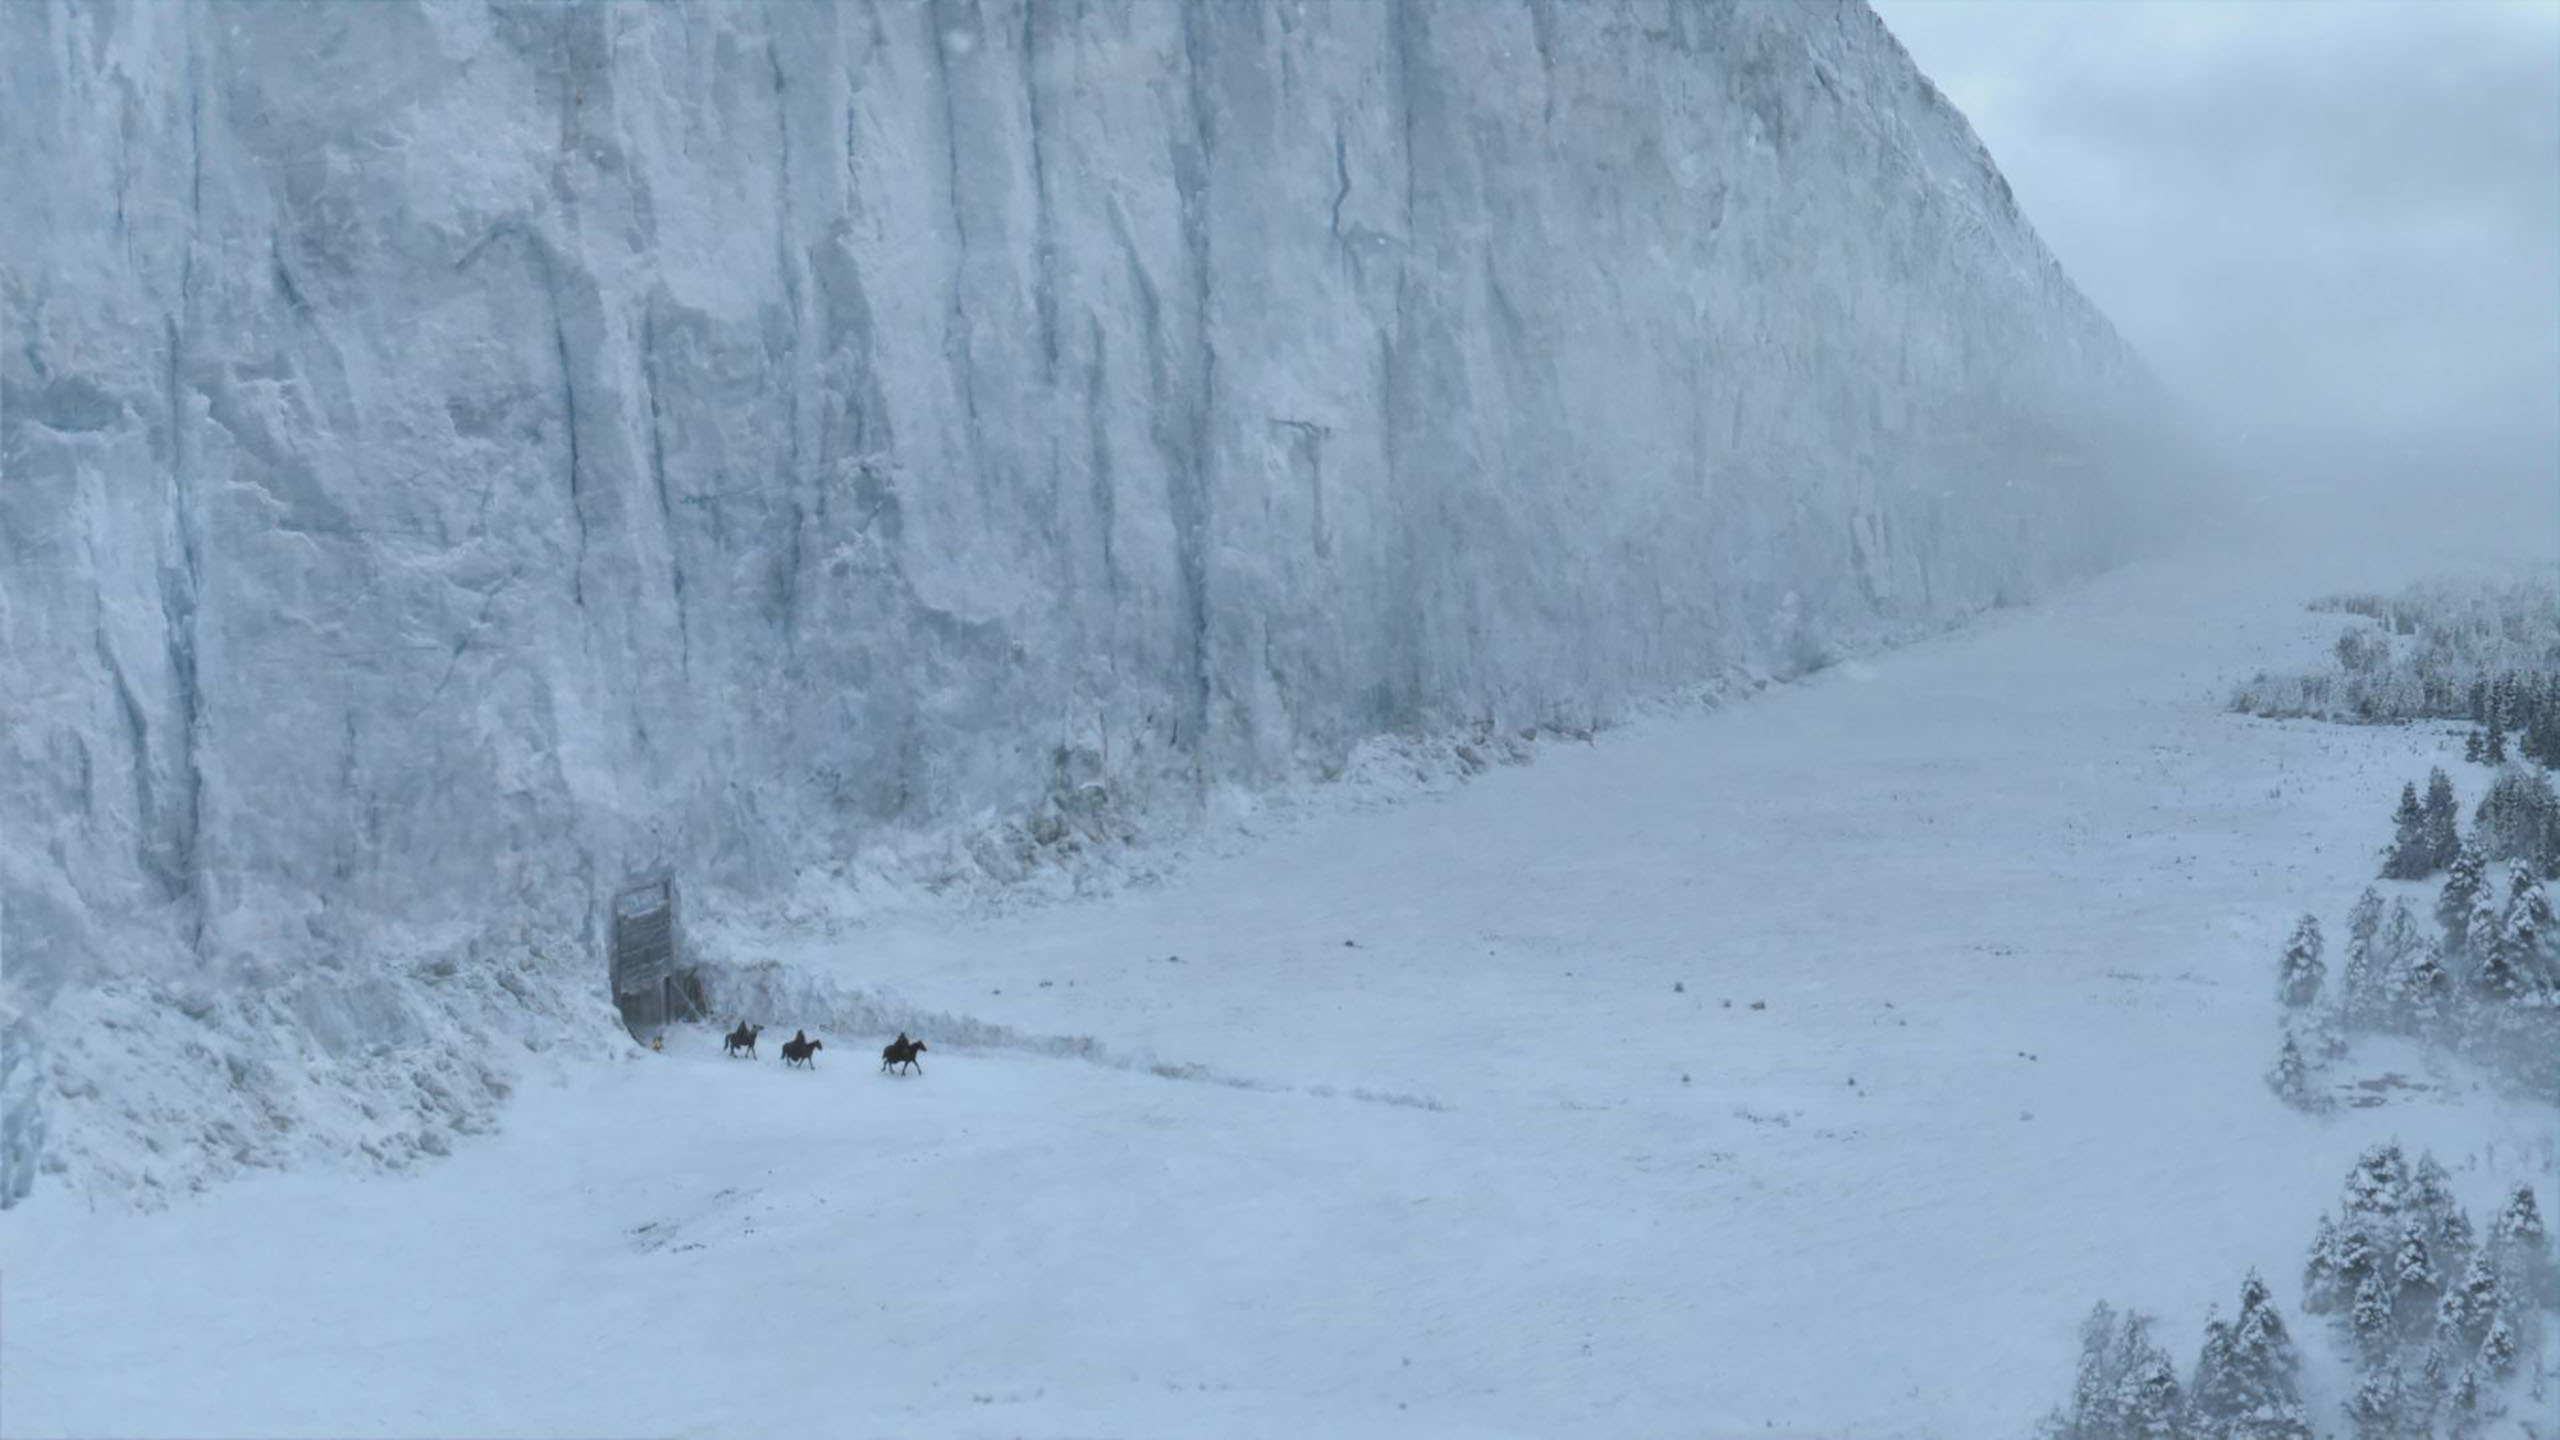
\includegraphics[height=6cm, width = 10cm]{./pic/wall.jpg}
				\caption{Na minha cabeça a Argentina é tipo wall de game of thrones!!!!}
				\label{fig_brincadeira}
		\end{figure}	
	\end{block}
\end{frame}

\begin{frame}	
	\begin{block}{Método científico}	
			\begin{itemize}
				\item Como essas duas perguntas se relacionam com essa apresentação?
			\end{itemize}
	\end{block}
\end{frame}


			